\documentclass[tikz,border=3pt]{standalone}
\usepackage[T1]{fontenc}
\usepackage[utf8]{inputenc}
\usepackage[english]{babel}
\usepackage{mathptmx}
\usepackage[scaled=0.92]{helvet}
\usepackage{amsmath,amssymb,textcomp}
\usetikzlibrary{positioning,arrows.meta}
\newcommand{\us}{\textmu s}
\begin{document}
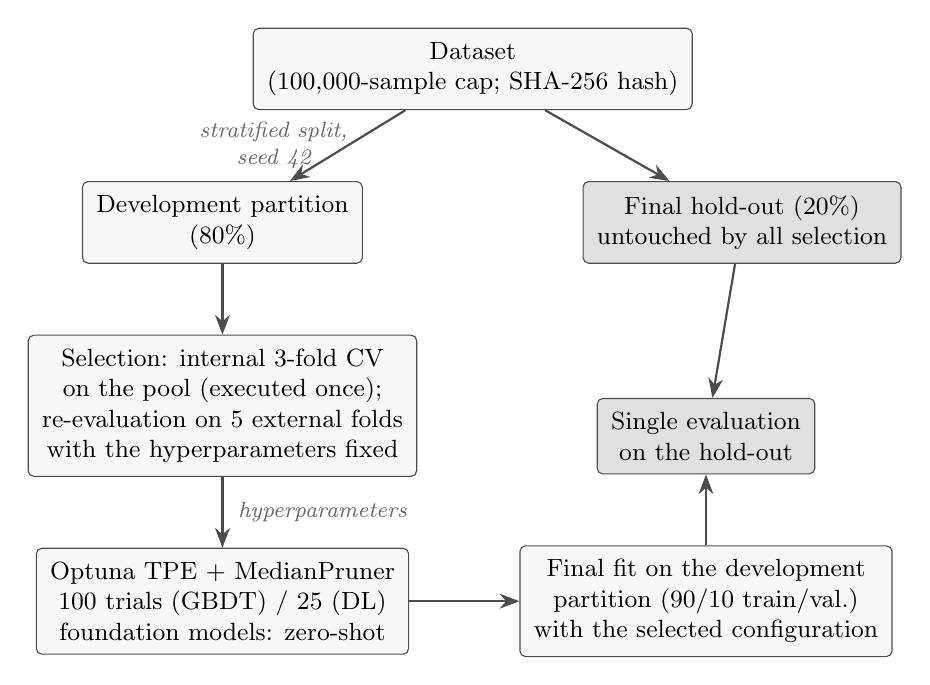
\begin{tikzpicture}[
  caixa/.style={draw=black!70, rounded corners=2pt, align=center,
    font=\small, inner sep=5pt, minimum height=9mm, fill=black!3},
  destaque/.style={caixa, fill=black!12},
  seta/.style={-{Stealth[length=2.5mm]}, thick, draw=black!70},
  rotulo/.style={font=\footnotesize\itshape, text=black!60, align=center},
  node distance=9mm and 8mm
]
\node[caixa] (dados) {Dataset\\(100{,}000-sample cap; SHA-256 hash)};
\node[caixa, below left=9mm and -14mm of dados] (dev)
  {Development partition\\(80\%)};
\node[destaque, below right=9mm and -14mm of dados] (hold)
  {Final hold-out (20\%)\\untouched by all selection};
\node[caixa, below=of dev] (nested)
  {Selection: internal 3-fold CV\\on the pool (executed once);\\re-evaluation on 5 external folds\\with the hyperparameters fixed};
\node[caixa, below=of nested] (optuna)
  {Optuna TPE + MedianPruner\\100 trials (GBDT) / 25 (DL)\\
   foundation models: zero-shot};
\node[caixa, right=14mm of optuna] (fit)
  {Final fit on the development\\partition (90/10 train/val.)\\
   with the selected configuration};
\node[destaque, above=of fit] (aval)
  {Single evaluation\\on the hold-out};
\draw[seta] (dados) -- node[rotulo, left=2pt, xshift=2mm] {stratified split,\\seed 42} (dev);
\draw[seta] (dados) -- (hold);
\draw[seta] (dev) -- (nested);
\draw[seta] (nested) -- node[rotulo, right=2pt] {hyperparameters} (optuna);
\draw[seta] (optuna) -- (fit);
\draw[seta] (fit) -- (aval);
\draw[seta] (hold) -- (aval);
\end{tikzpicture}
\end{document}
